\section{Real Analysis}

This section develops the real-sequence notions of convergence and limit superior and inferior, together with the basic definition of a series. These topics follow the treatment of the real numbers and convergence in \cite[Chapter 1, Sections 1.8 and 1.16]{Berberian1998-qc}.

\subsection{Sequences and Convergence}

\begin{definition}[Sequence]
A real sequence is a function $a:\mathbb{N}\to\mathbb{R}$. Its value at $n$ is denoted by $a_n$, and the sequence is written $(a_n)_{n\geq 1}$ or simply $(a_n)$.
\end{definition}

\begin{definition}[Convergence]
A sequence $(a_n)$ converges to $L\in\mathbb{R}$ if for every $\varepsilon>0$ there is an integer $N$ such that
\[
 n\geq N\quad\Longrightarrow\quad |a_n-L|<\varepsilon.
\]
In this case, $L$ is called the limit of the sequence and we write $a_n\to L$.
\end{definition}

\begin{figure}[htbp]
\centering
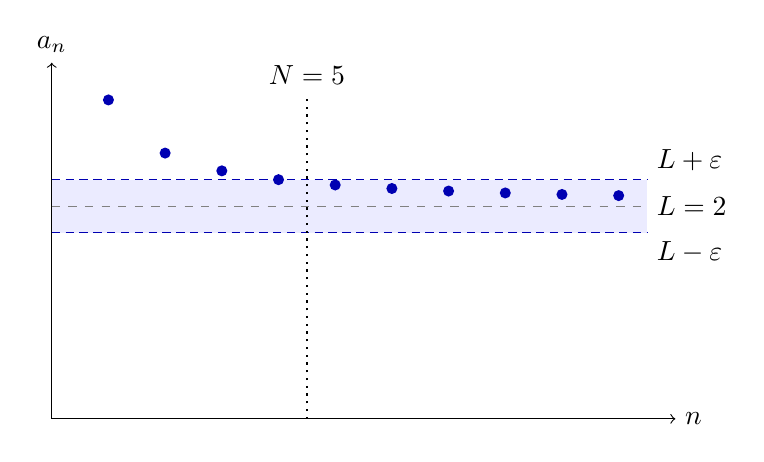
\begin{tikzpicture}[x=0.72cm,y=1.35cm]
    \fill[blue!8] (0,1.75) rectangle (10.5,2.25);
    \draw[->] (0,0) -- (11,0) node[right] {$n$};
    \draw[->] (0,0) -- (0,3.35) node[above] {$a_n$};
    \draw[dashed,gray] (0,2) -- (10.5,2) node[right,black] {$L=2$};
    \draw[densely dashed,blue!70!black] (0,2.25) -- (10.5,2.25) node[right,black,yshift=7pt] {$L+\varepsilon$};
    \draw[densely dashed,blue!70!black] (0,1.75) -- (10.5,1.75) node[right,black,yshift=-7pt] {$L-\varepsilon$};
    \draw[dotted,thick] (4.5,0) -- (4.5,3.05) node[above] {$N=5$};
    \foreach \n/\y in {1/3,2/2.5,3/2.333,4/2.25,5/2.2,6/2.167,7/2.143,8/2.125,9/2.111,10/2.1} {
        \fill[blue!70!black] (\n,\y) circle (2pt);
    }
\end{tikzpicture}
\caption{The sequence $a_n=2+1/n$ approaches $L=2$. For $\varepsilon=0.25$, all terms with $n\geq5$ lie inside the shaded band.}
\label{fig:sequence-convergence}
\end{figure}

\begin{theorem}[Uniqueness of limits]
A convergent real sequence has exactly one limit.
\end{theorem}

\begin{proof}
Suppose $a_n\to L$ and $a_n\to M$. For any $\varepsilon>0$, choose an index after which both $|a_n-L|<\varepsilon/2$ and $|a_n-M|<\varepsilon/2$. The triangle inequality gives
\[
 |L-M|\leq |L-a_n|+|a_n-M|<\varepsilon.
\]
Since this holds for every positive $\varepsilon$, $|L-M|=0$ and hence $L=M$.
\end{proof}

\begin{theorem}[Convergent sequences are bounded]
Every convergent real sequence is bounded.
\end{theorem}

\begin{proof}
Let $a_n\to L$. Taking $\varepsilon=1$, there is an index $N$ such that $|a_n-L|<1$ for every $n\geq N$. Thus $|a_n|<|L|+1$ for all such $n$. The finitely many terms $a_1,\ldots,a_{N-1}$ are also bounded, so the entire sequence is bounded.
\end{proof}

\clearpage

\begin{definition}[Cauchy sequence]
A real sequence $(a_n)$ is a Cauchy sequence if for every $\varepsilon>0$ there is an integer $N$ such that
\[
 m,n\geq N\quad\Longrightarrow\quad |a_m-a_n|<\varepsilon.
\]
\end{definition}

\begin{figure}[H]
\centering
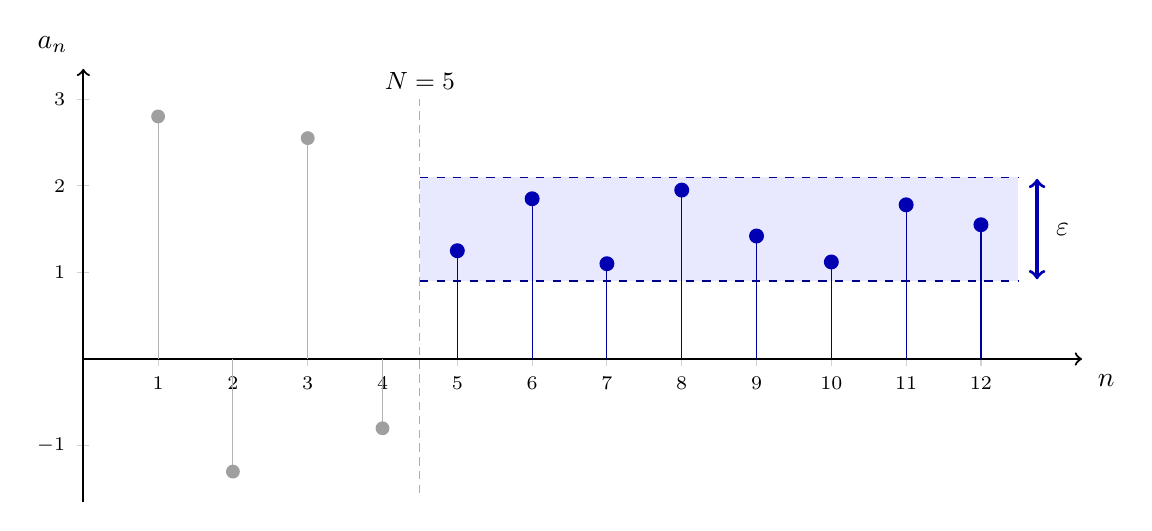
\begin{tikzpicture}[x=0.95cm,y=1.1cm]
    \path[fill=blue!9] (4.5,0.9) rectangle (12.5,2.1);
    \draw[blue!55!black,dashed] (4.5,0.9) -- (12.5,0.9);
    \draw[blue!55!black,dashed] (4.5,2.1) -- (12.5,2.1);
    \draw[gray!65,densely dashed] (4.5,-1.55) -- (4.5,3.0);
    \node[above,font=\small] at (4.5,3.0) {$N=5$};
    \draw[<->,very thick,blue!70!black] (12.75,0.92) -- (12.75,2.08)
        node[midway,right=3pt,black] {$\varepsilon$};

    \foreach \n in {1,...,12} {
        \draw[gray!35] (\n,0) -- (\n,-0.08);
        \node[below=3pt,font=\scriptsize] at (\n,0) {$\n$};
    }
    \foreach \y in {-1,1,2,3} {
        \draw[gray!35] (0.08,\y) -- (-0.08,\y);
        \node[left=3pt,font=\scriptsize] at (0,\y) {$\y$};
    }
    \draw[->,thick] (0,0) -- (13.35,0) node[below right=2pt] {$n$};
    \draw[->,thick] (0,-1.65) -- (0,3.35) node[above left=2pt] {$a_n$};

    \foreach \n/\value in {1/2.8,2/-1.3,3/2.55,4/-0.8} {
        \draw[gray!60] (\n,0) -- (\n,\value);
        \fill[gray!75] (\n,\value) circle (2.5pt);
    }
    \foreach \n/\value in {5/1.25,6/1.85,7/1.1,8/1.95,9/1.42,10/1.12,11/1.78,12/1.55} {
        \draw[blue!60!black] (\n,0) -- (\n,\value);
        \fill[blue!70!black] (\n,\value) circle (2.7pt);
    }
\end{tikzpicture}
\caption{Illustration of the Cauchy condition for a chosen $\varepsilon$: from $N=5$ onward, all plotted terms lie strictly between two levels separated by $\varepsilon$, so any two tail terms differ by less than $\varepsilon$.}
\label{fig:cauchy-sequence-tail}
\end{figure}

\begin{proposition}
Every convergent real sequence is a Cauchy sequence.
\end{proposition}

\begin{proof}
Suppose $a_n\to L$. Given $\varepsilon>0$, choose $N$ such that $|a_n-L|<\varepsilon/2$ for every $n\geq N$. If $m,n\geq N$, then
\[
 |a_m-a_n|\leq |a_m-L|+|a_n-L|<\varepsilon.
\]
Therefore $(a_n)$ is Cauchy.
\end{proof}

\subsection{Limit Superior and Limit Inferior}

For a bounded real sequence, each tail has a supremum and an infimum. The supremum of the tails decreases as the starting index increases, while the infimum of the tails increases.

\begin{definition}[Limit superior and limit inferior]
For a bounded real sequence $(a_n)$, define
\[
 \limsup_{n\to\infty}a_n=\inf_{N\geq1}\sup_{n\geq N}a_n,
 \qquad
 \liminf_{n\to\infty}a_n=\sup_{N\geq1}\inf_{n\geq N}a_n.
\]
\end{definition}

\begin{theorem}
For every bounded real sequence $(a_n)$,
\[
 \liminf_{n\to\infty}a_n\leq\limsup_{n\to\infty}a_n.
\]
Moreover, $(a_n)$ converges if and only if these two quantities are equal; when they are equal, their common value is the limit of $(a_n)$.
\end{theorem}

\begin{proof}
For any two indices $M,N$, the tails beginning at $M$ and $N$ have a common term $a_k$ when $k\geq\max\{M,N\}$. Consequently,
\[
 \inf_{n\geq M}a_n\leq a_k\leq\sup_{n\geq N}a_n.
\]
Taking the supremum over $M$ on the left and the infimum over $N$ on the right proves the inequality.

If $a_n\to L$, then for every $\varepsilon>0$ all sufficiently late terms lie between $L-\varepsilon$ and $L+\varepsilon$. The tail infima and suprema, and therefore their respective limits, lie in the same interval. Since this holds for every $\varepsilon>0$, both are $L$.

Conversely, suppose both quantities equal $L$. For any $\varepsilon>0$, the definition of the infimum of the tail suprema gives an index $N_1$ for which $\sup_{n\geq N_1}a_n<L+\varepsilon$. The definition of the supremum of the tail infima gives an index $N_2$ for which $\inf_{n\geq N_2}a_n>L-\varepsilon$. For $n\geq\max\{N_1,N_2\}$, these bounds imply $L-\varepsilon<a_n<L+\varepsilon$. Hence $a_n\to L$.
\end{proof}

\begin{figure}[htbp]
\centering
\begin{tikzpicture}[x=0.62cm,y=1.15cm]
    \draw[->] (0,0) -- (13,0) node[right] {$n$};
    \draw[->] (0,-1.25) -- (0,1.75) node[above] {$a_n$};
    \draw[dashed,red!70!black] (0,1) -- (12.5,1) node[right,black] {$\limsup a_n=1$};
    \draw[dashed,blue!70!black] (0,-1) -- (12.5,-1) node[right,black] {$\liminf a_n=-1$};
    \foreach \n/\y in {1/0,2/1.5,3/-0.667,4/1.25,5/-0.8,6/1.167,7/-0.857,8/1.125,9/-0.889,10/1.1,11/-0.909,12/1.083} {
        \draw[gray!65] (\n,0) -- (\n,\y);
        \fill[black] (\n,\y) circle (2pt);
    }
\end{tikzpicture}
\caption{For $a_n=(-1)^n+1/n$, the even and odd subsequences approach $1$ and $-1$, respectively.}
\label{fig:limsup-liminf}
\end{figure}

\subsection{Series}

\begin{definition}[Series and partial sums]
Given a real sequence $(a_n)$, its $N$th partial sum is
\[
 S_N=\sum_{n=1}^{N}a_n.
\]
The series $\sum_{n=1}^{\infty}a_n$ converges to $S$ if the sequence of partial sums $(S_N)$ converges to $S$. Otherwise, the series diverges.
\end{definition}

\begin{figure}[htbp]
\centering
\begin{tikzpicture}[x=0.78cm,y=3.0cm]
    \draw[->] (0,0) -- (8,0) node[right] {$N$};
    \draw[->] (0,0) -- (0,1.18) node[above] {$S_N$};
    \draw[dashed,red!70!black] (0,1) -- (7.6,1) node[right,black] {$S=1$};
    \foreach \n/\s in {1/0.5,2/0.75,3/0.875,4/0.9375,5/0.96875,6/0.984375,7/0.9921875} {
        \draw[gray!65] (\n,0) -- (\n,\s);
        \fill[blue!70!black] (\n,\s) circle (2pt);
    }
\end{tikzpicture}
\caption{The partial sums $S_N=\sum_{n=1}^{N}2^{-n}=1-2^{-N}$ approach the sum $1$.}
\label{fig:series-partial-sums}
\end{figure}

\begin{theorem}[Necessary condition for convergence]
If $\sum_{n=1}^{\infty}a_n$ converges, then $a_n\to0$.
\end{theorem}

\begin{proof}
Let $S_N=\sum_{n=1}^{N}a_n$ and suppose $S_N\to S$. For $n\geq2$, $a_n=S_n-S_{n-1}$. Both partial-sum sequences on the right tend to $S$, so
\[
 a_n=S_n-S_{n-1}\longrightarrow S-S=0.
\]
\end{proof}

\begin{example}[Geometric series]
For a real number $r$ with $|r|<1$, the finite partial sums satisfy
\[
 \sum_{n=0}^{N}r^n=\frac{1-r^{N+1}}{1-r}.
\]
Since $r^{N+1}\to0$, the geometric series converges and
\[
 \sum_{n=0}^{\infty}r^n=\frac{1}{1-r}.
\]
\end{example}